This chapter describes how we have implemented the different elements of our game. It describes how we load and draw the texture for the train, how we have implemented the wheels and train smoke in order to create the illusion that the train is moving between the stations and how we randomly generate the background elements.

%drag and drop section
\section{Drag and Drop}
As mentioned in \secref{sec:androiddraganddrop}, the implementation of drag and drop has been simplified after SDK 11. This allows for an easy implementation of the drag and drop functionality. Before the explanation of drag and drop, we will first show the hierarchy of the layouts on the station and the wagons.
\begin{figure}[H]
\centering
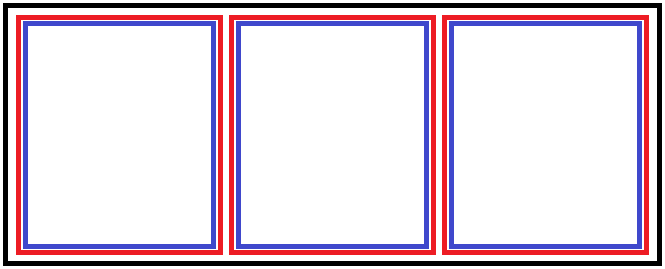
\includegraphics[width=0.9\linewidth]{img/layoutexample.png}%0.1 margin
\caption{Example of a LinearLayout container.}
\label{fig:linearlayoutcontainer}
\end{figure}
There are two LinearLayout containers on each station, and there are a LinearLayout containers on each wagon. An example of the LinearLayout container is shown in \autoref{fig:linearlayoutcontainer}. The black color represents the LinearLayout, the red color represents a Framelayout, and the blue color represents a pictogram. Each pictogram has attached an OnTouchListener, and each FrameLayout has attached an OnDragListener. Our TouchListener is shown below.

\begin{lstlisting}[language=java,firstnumber=1,caption={Our TouchListener},label=lst:ourtouchlistener] 
private final class TouchListener implements OnTouchListener {
	@Override
	public boolean onTouch(View view, MotionEvent motionEvent) {
		if (motionEvent.getAction() == MotionEvent.ACTION_DOWN) {
			ClipData data = ClipData.newPlainText("", "");
			DragShadowBuilder shadowBuilder = new View.DragShadowBuilder(view);
			view.startDrag(data, shadowBuilder, view, 0);
			view.setVisibility(View.INVISIBLE);
			return true;
		}
		else if (motionEvent.getAction() == MotionEvent.ACTION_UP) {// prevents that a pictogram disappears if only pressed and no drag
			if(view != null && view.getVisibility() == View.INVISIBLE){
				view.setVisibility(View.VISIBLE);
			}
			return true;
		}
		else {
			return false;
		}
	}
}
\end{lstlisting}
\begin{description}
\item[Line 3] The \lstinline|onTouch()| method is called when the pictograms receives a touch input.
\item[Lines 4-7] If the touch event is a press motion, make a view shadow, and start the drag.
\item[Line 8] Set the pictogram's visibility to invisible.
\item[Lines 11-14] If the touch event is a release motion and the pictogram is invisible, then make the pictogram visible. This if sentence was added since it was possible to make the pictogram disappear with only a press motion.
\todo{Der er nødt til at stå hvorfor den returnerer true/false}
\end{description}
When the method \textit{view.startDrag()} is called, the OnDragListener event is fired. Our OnDragListener is shown below.
\begin{lstlisting}[language=java,firstnumber=1,caption={Our DragListener},label=lst:ourdraglistener] 
private class DragListener implements OnDragListener {
	public boolean onDrag(View hoverView, DragEvent event) {
	    View draggedView = (View) event.getLocalState();
			switch (event.getAction()) {
				case DragEvent.ACTION_DROP:
					// DropAction, assigns the draggedview to the dropContainer if, the dropContainer does not already contain a pictogram.
					ViewGroup ownerContainer = (ViewGroup) draggedView.getParent();
					PictoFrameLayout dropContainer = (PictoFrameLayout) hoverView;
					Object tag = hoverView.getTag();
					if (tag == null) {
						ownerContainer.removeView(draggedView);
						ownerContainer.setTag(null);
						dropContainer.addView(draggedView);
						dropContainer.setTag("filled");
					}
					draggedView.setVisibility(View.VISIBLE);
					break;

				case DragEvent.ACTION_DRAG_ENDED:
					// Makes the draggedview visible again after the view has been moved or if drop wasn't valid.
					if(event.getResult() == false){
						draggedView.setVisibility(View.VISIBLE);
					}
					break;
			}
			return true;
	}
}
\end{lstlisting}
\begin{description}
\item[Line 2] The \lstinline|onDrag()| method is called when a pictogram starts being dragged.
\item[Line 3] Get the current dragged pictogram and initialize the variable \lstinline|draggedView|.
\item[Line 4] Switch case of the current drag event.
\item[Line 5] Case if the current drag event is dropping the pictogram on a FrameLayout.
\item[Lines 7-8] Initialize the variable \lstinline|ownerContainer| with the parent Framelayout of the dragged pictogram, and initialize variable \lstinline|dropContainer| with the FrameLayout currently being hovered above.  
\item[Lines 9-10] Initialize the variable \textit{tag} with the current status of the \lstinline|dropContainer|, if the status is "filled" then the \lstinline|dropContainer| is already containing a pictogram, and is therefore not eligible for the drop.
\item[Lines 11-16] If the \lstinline|dropContainer| does not contain a pictogram, then the pictogram can be moved from \lstinline|ownerContainer| to \lstinline|dropContainer|. The tag in \lstinline|ownerContainer| is set to \lstinline|null| and the tag in \lstinline|dropContainer| is set to \lstinline|"filled"|, to indicate to it now contains a pictogram. The \lstinline|draggedView| becomes visible after a drop.
\item[Line 19] If current drag event is drag ended,  there were not performed a valid drop the \lstinline|draggedView| will become visible again. This will make it look like the pictogram snaps back to its position, since the drop was not valid.
\end{description}
Some cases has been excluded in \autoref{lst:ourdraglistener} because they are not relevant for the functionality of the drag and drop.


\section{Train \& Wagons}
The train and wagons are stationary textures on the tablet screen, it is actually the background that moves in order to create the illusion that the train is driving. \autoref{lst:loadtexture} shows how we load the texture for our train and wagons.

\begin{lstlisting}[language=java,firstnumber=1,caption={Loading the texture for our train and wagons.},label=lst:loadtexture] 
	// Initialize a train object and a wagon object
	private final Texture train = new Texture(1.0f, 1.0f);
	private final Texture wagon = new Texture(1.0f, 1.0f);

	//Load the textures
	this.wagon.loadTexture(R.drawable.texture_wagon, AspectRatio.BitmapOneToOne);
	this.train.loadTexture(R.drawable.texture_train, AspectRatio.BitmapOneToOne); 
\end{lstlisting}

\begin{description}
\item[Lines 2-3] Initialising the \lstinline|train| and \lstinline|wagon| objects, with the size $1 \times 1$.
\item[Line 6] This loads the \lstinline|wagon| texture, \lstinline|R.drawable.texture_wagon| defines which texture gets loaded, which in this case is the wagon and \lstinline|AspectRatio.BitmapOneToOne| makes sure the texture keeps the original aspect ratio by resize the texture, as described in \secref{sec:openglimp}.
\item[Line 7] This loads the \lstinline|train| texture, and the original aspect ratio is kept again.
\end{description}

Now the texture is successfully loaded we have to place it on right location on the tablet screen. This is done using the coordinate system mentioned in \secref{sec:frustum}. This is done as shown in \autoref{lst:addcoordinate}.

\begin{lstlisting}[language=java,firstnumber=1,caption={Placing the texture on the screen.},label=lst:addcoordinate] 
	//Add coordnates to the renderables
	this.wagon.addCoordinate(-542.32f, -142.72f, GameData.FOREGROUND);
	this.wagon.addCoordinate(-187.45f, -142.72f, GameData.FOREGROUND);
	this.train.addCoordinate(160.42f, -52.37f, GameData.FOREGROUND);
\end{lstlisting}

\begin{description}
\item[Lines 2-3] We have chosen to have two wagons on our train, but we only have one wagon object with two coordinates. \lstinline|GameData.Foreground| determines the depth in the frustum where the objects are placed.
\item[Line 4] Adds a coordinate for the placement of the \lstinline|train|.
\end{description}

Now the textures have been loaded and given coordinates, they are ready to be drawn. This is done as shown in \autoref{lst:drawtexture}

\begin{lstlisting}[language=java,firstnumber=1,caption={Drawing the texture on the screen.},label=lst:drawtexture] 
	//Drawing the textures
	super.translateAndDraw(this.wagon);
	super.translateAndDraw(this.train);
\end{lstlisting}

\begin{description}
\item[Lines 2-3] This draws the \lstinline|wagon| and \textit{train} objects. The \lstinline|translateAndDraw| method is explained in \secref{sec:gamerendering}
\end{description}

\subsection{Wheels}

To create the illusion that the train is moving, we had to make wheels rotate in order to make it look like it was actually driving. 

The wheels are loaded and given a coordinate in the same way as the train that was just explained.

The difference comes when the wheels are drawn, we have to rotate the wheels so that it looks like the train moves, this is done by calculating the rotation using the function shown in \autoref{lst:calcrotate}.

\begin{lstlisting}[language=java,firstnumber=1,caption={Rotating and drawing the wheels.},label=lst:calcrotate]
    private float[] rotation = { 0f, 0f, 0f }; // rotation number for each wheel size
    private final double[] wheelDiameter = {
            106.39f, // large wheel
            78.71f,  // medium wheel
            60.8f    // small wheel
    };

    private final float calculateRotation(int wheelIndex) {    
        float circumference = this.wheelDiameter[wheelIndex] * Math.PI;
        float degreePerPixel = 360.0 / circumference;
        this.rotation[wheelIndex]+= degreePerPixel * super.gameData.getPixelMovement();
        return this.rotation[wheelIndex];
    }
\end{lstlisting}

\begin{description}
\item[Line 1] This array has the rotation number for each wheel size.
\item[Lines 2-6] This array has the diameter in pixels for each wheel size. 
\item[Line 8] The function takes a wheelIndex as parameter, this is to determine which the wheel size that is being used for calculations. 
\item[Line 9] The wheel's circumference is being calculated.
\item[Line 10] Calculating the degreePerPixel by dividing 360 with the circumference
\item[Line 11] Here the rotation for the specific wheel is calculated by taking the degreePerPixel we just found and multiplying it by the pixel movement. \lstinline|GameData.getPixelMovement| is explained in \secref{sec:gamerendering}. Please note that the rotation is not reset, it keeps getting added to, however is it is not necessary to reset it as the rotation will not reach an overflow.
\item[Line 12] The specific wheel's rotation is returned. 
\end{description}

This function is called each time a wheel is drawn. This is done by using \lstinline|translateRotateAndDraw| as can be seen in \autoref{lst:rotatewheels}

\begin{lstlisting}[language=java,firstnumber=1,caption={Rotating and drawing the wheels.},label=lst:rotatewheels]
	// Rotate and draw the wheels
super.translateRotateAndDraw(this.calculateRotation(this.mediumWheelIndex), this.mediumWheel);
super.translateRotateAndDraw(this.calculateRotation(this.largeWheelIndex), this.largeWheel);
super.translateRotateAndDraw(this.calculateRotation(this.smallWheelIndex), this.smallWheel);
\end{lstlisting}

\begin{description}
\item[Lines 2-4] Each time a wheel has to be drawn, \lstinline|calculateRotation| with the specific wheelIndex as parameter, is called and the rotation is calculated. The wheel is rotated and then drawn. 
\end{description}

\subsection{Train smoke}

Another element in making it look like the train is moving is the train smoke. While the train is standing still at the station the smoke goes vertically up in the air, but when the train moves the smoke moves horizontally. 

The smoke clouds are reset and updated based on time, as can be seen in \autoref{lst:cloudstime}

\begin{lstlisting}[language=java,firstnumber=1,caption={Smoke clouds getting reset based on time intervals.},label=lst:cloudstime]
//Reset one smoke cloud at the given interval
this.timeSinceLastReset += super.gameData.timeDifference;
if (this.timeSinceLastReset >= this.timeBetweenSmokeClouds) {
    this.timeSinceLastReset = 0f;
    
    if (!super.gameData.isPaused) {
        this.resetOneSmokeCloud();
    }
}

if (!super.gameData.isPaused) {
    //Update position and alpha channels
    this.updateSmokeClouds();
}
\end{lstlisting}

\begin{description}
\item[Line 2] The \lstinline|timeSinceLastReset| is the time since a smoke cloud was last reset and \lstinline|gameData.timeDifference| is the time that has elapsed, in milliseconds. 
\item[Lines 2-9] If the time since last reset is higher or equal to the time between the smoke clouds (this is a variable we have pre-determined), then \lstinline|timeSinceLastReset| is set to 0, and if the game is not paused, then the smoke cloud is reset back to its starting position. 
\item[Lines 11-14] If the game is not paused, then the smoke cloud's coordinates are updated, in order to move the smoke cloud. 
\end{description}

\autoref{lst:cloudstime} showed two methods, \lstinline|resetOneSmokeCloud| and \lstinline|updateSmokeClouds|. These are the two methods in charge of updating and resetting the smoke cloud's positions, making it look like they move. They are explained in \autoref{lst:resetonesmokecloud} and \autoref{lst:updatesmokeclouds}

\begin{lstlisting}[language=java,firstnumber=1,caption={Smoke clouds getting reset based on time intervals.},label=lst:resetonesmokecloud]
private final void resetOneSmokeCloud() {
    //Increment the reset index
    this.resetIndex = ++this.resetIndex % this.numberOfSmokeClouds;
    
    //Put cloud back to exhaust
    this.coordinates[this.resetIndex].setCoordinate(this.startCoordinate.getX(), this.startCoordinate.getY());
    this.colors[this.resetIndex].setColor(1f, 1f, 1f, 1f);
}
\end{lstlisting}

\begin{description}
\item[Line 3] This resets the index, helping to keep track of which cloud that has to be reset. 
\item[Lines 6-7] This resets the specific cloud back to its starting position and it also resets the color back to its original. 
\end{description}
 
\begin{lstlisting}[language=java,firstnumber=1,caption={Smoke clouds getting reset based on time intervals.},label=lst:updatesmokeclouds]
private final void updateSmokeClouds() {
    //Updates position and alpha channels
    for (int i = 0; i < this.numberOfSmokeClouds; i++) {
        //Always move smoke vertically, move smoke horizontally relative to the train speed.
        this.coordinates[i].moveX(super.gameData.getPixelMovement());
        this.coordinates[i].moveY(this.ySpeed * super.gameData.timeDifference);
        
        //Fade the smoke
        this.colors[i].alpha -= (1f / (this.timeBetweenSmokeClouds * this.numberOfSmokeClouds)) * super.gameData.timeDifference;
    }
}
\end{lstlisting}

\begin{description}
\item[Lines 3-6] This is in charge of moving the clouds. The clouds are moved on both the x and y axis. The new x coordinate depends on \lstinline|gameData.getPixelMovement| which is explained in \secref{sec:gamerendering}. The new y coordinate depends on a constant called \lstinline|ySpeed|, and \lstinline|gameData.timeDifference|, which is the time that has elapsed.
\item[Line 9] This fades the smoke clouds. The cloud's original alpha channel is one, and each time the smoke cloud is updated and moved, the alpha color lowered, making the cloud more see-through, to make it look like they disappear up in the air. 
\end{description}

\section{Station}

We have made three different station textures and to ensure an element of surprise in our game, each time we start the game we shuffle the list of stations so the order always will be random, however this only happens when the game is started, so the order within the same game is the same. \autoref{lst:stations} shows this implementation.
 
\begin{lstlisting}[language=java,firstnumber=1,caption={Smoke clouds getting reset based on time intervals.},label=lst:stations]
Collections.shuffle(stations);
LinkedList<StationContainer> stationsQueue = this.getQueue(stations);

float xPosition = -364f; // first platform position

for (int i = 0; i < super.gameData.numberOfStations; i++) {
    StationContainer nextStation = stationsQueue.pop();
    stationsQueue.add(nextStation);
    this.stationPlatformMatrix.addRenderableMatrixItem(nextStation.station, new Coordinate(xPosition + nextStation.xOffset, nextStation.yOffset, 0f));
    
    xPosition += GameData.DISTANCE_BETWEEN_STATIONS;        
    
}
\end{lstlisting}

\begin{description}
\item[Lines 1-2]  The stations are shuffled and added to the queue.
\item[Line 4] \lstinline|xPosition| is the position in which the platform will be drawn. 
\item[Line 7-8] The next station is found and popped off the queue, and added to the end of the queue again to ensure there are always are stations in the queue. 
\item[Line 9] The station is drawn in the correct position.\todo{Omskriv og uddyb! Der står ikke at vi bruger en station matrix.}
\item[Line 11] \lstinline|xPosition| is updated with the pre-determined distance between stations to ensure each station has the same distance between them. This is especially important when we have to calculate when the train has to stop. 
\end{description}

\subsection{Stopping position}

In order for us to stop the train at the correct location each time, we have to calculate the stopping position, this is done as shown in \autoref{lst:nextstopping}.

\begin{lstlisting}[language=java,firstnumber=1,caption={Smoke clouds getting reset based on time intervals.},label=lst:nextstopping]
public final void calculateStoppingPositions() {        
    //Make new array
    super.gameData.nextStoppingPosition = new float[super.gameData.numberOfStations + 1];
    
    //Calculate all stopping positions
    super.gameData.nextStoppingPosition[0] = GameData.DISTANCE_BETWEEN_STATIONS;
    for (int i = 1; i < super.gameData.numberOfStations; i++) {
        super.gameData.nextStoppingPosition[i] += super.gameData.nextStoppingPosition[i-1] + GameData.DISTANCE_BETWEEN_STATIONS;
    }
}
\end{lstlisting}

\begin{description}
\item[Line 2] An array for the stopping positions is initialized. \todo{Vi laver +1 fordi Train Depot også er med i array'et, train depot stoppested bliver tilføjet i train depot filen, skriv}
\item[Line 6] The first stopping position is equal to the pre-determined distance between station. 
\item[Lines 7-9] We loop through the array and calculate the next stopping position for all stations. This is done by adding the distance to the next station to the stopping position of the previous station.
\end{description}

\section{Game background}

The background for our game is randomly generated for each game session as mentioned in \secref{sec}\todo{Mangler en ref}. 

\subsection{Hills}

We have created four different sequences of hills, each sequence consists of four hills in a specific layout. This four sequences are randomly chosen throughout the game and is random each time. It is important to note that every hill texture is only loaded once, even though it is used multiple times in the game. \autoref{lst:hills} shows one of the hill sequences.\todo{Forklar kort hvad HillItem er, og skriv hvad constructoren tager i mod.}

\begin{lstlisting}[language=java,firstnumber=1,caption={Hill sequence.},label=lst:hills]
HillItem[] hillSequence1 = {
    new HillItem(0f, this.hill_large.getHeight(), this.hill_large),
    new HillItem(this.hill_large.getWidth()+11f, this.hill_medium.getHeight(), this.hill_medium),
    new HillItem(this.hill_large.getWidth()/100f*60f, this.hill_small.getHeight(), this.hill_small),
    new HillItem(this.hill_large.getWidth()+11f + this.hill_medium.getWidth()/100f*65f, this.hill_larger.getHeight(), this.hill_larger)
};
\end{lstlisting}

\begin{description}
\item[Line 2] As a starting point our hills are placed in the bottom left corner, so the first hill has the x-coordinate of 0, and because we draw the texture from the top left corner, we ensure that the hill is placed correctly by making the y-coordinate equal the height of the hill. 
\item[Line 3] The next hill is placed relative to the first hill, the x-coordinate is the width of the hill that came before it plus a constant. The y-coordinate equals the height of the hill again.
\item[Line 4] The x-coordinate for the third hill is a percentage of the width of the first hill. 
\item[Line 5] The last hill is placed relative to the first two hills.
\end{description}

An important thing to note about the placement of the hills is the order in which they are added to the sequence, The hill furthest to the back has to be drawn first, then the second furthest and so on. This is also why the third hill in the sequence is drawn with a smaller x-coordinate than the second hill in the sequence.

\subsection{Trees \& Cows}

The trees and cows are randomly generated as well, however they are implemented in a very special way. 

We have an array consisting of the cow texture and the tree texture, we then have several random factors that play in before we find what to place and where to place it. 

First we randomly choose which of the four hill sequences we want to draw on, this is because we do not want cows and trees on every hill sequences as they are meant to be an element of surprise for the player. 

Now we know which hill sequence we draw on, we have to find out what to draw, this is also chosen randomly. We now know what to draw and on which hill sequence to draw it, but we still need to find out which hill in that sequence to draw it on, because we do not want to draw on every hill in the specific sequence. This is again chosen with a random number. We have set up four cases, one for each type of hill. Before a cow or a tree is drawn the random number we picked has to match the specific hill being drawn at that moment in time. 

For example if we have to draw a cow and the random number picked is one, which means we have to draw the cow on a medium hill, but the current hill is a large, then the cow will not be drawn. On the other hand if the current hill was a medium hill, then the cow would be drawn on a random location on this hill. For a full view of what this looks like in the game, look in \autoref{app:}\todo{Mangler section med billeder i Appendix} \todo{Der mangler noget forklaring her, hvad er 'current hill'?}

\subsection{Clouds \& sun}

The clouds are also implemented with a degree of randomness. There will always be clouds on the sky, however the speed and placement on the sky is random to a certain degree. 

The clouds move on the x-axis with a random velocity between $0.07$ and $0.18$ pixels per millisecond, the clouds are also randomly placed on the top 1/4th of the screen. 

The sun is a stationary texture in the top right corner of the screen. 